\subsection{Прецессия}

Под действием возмущающих сил ось вращения Земли совершает прецессионное движение: описывает вокруг оси эклиптики конус с углом раствора $23.5^\circ$ с периодом около  25\,765~лет. Из-за этого меняется положение полюс мира. Например, сейчас полюс мира практически совпадает с Полярной звездой ($\alpha$\,UMi), а 15\,000~лет назад роль полярной звезды играла Вега ($\alpha$\,Lyr). Если считать, что величина прецессии постоянна, то полюсы мира описывают вокруг полюсов эклиптики малые круги с радиусом $23.5^\circ$. В действительности же величина прецессии меняется, поэтому путь полюсов мира представляет собой не окружность, а спираль.

\begin{wrapfigure}[16]{r}{0.5\tw}
	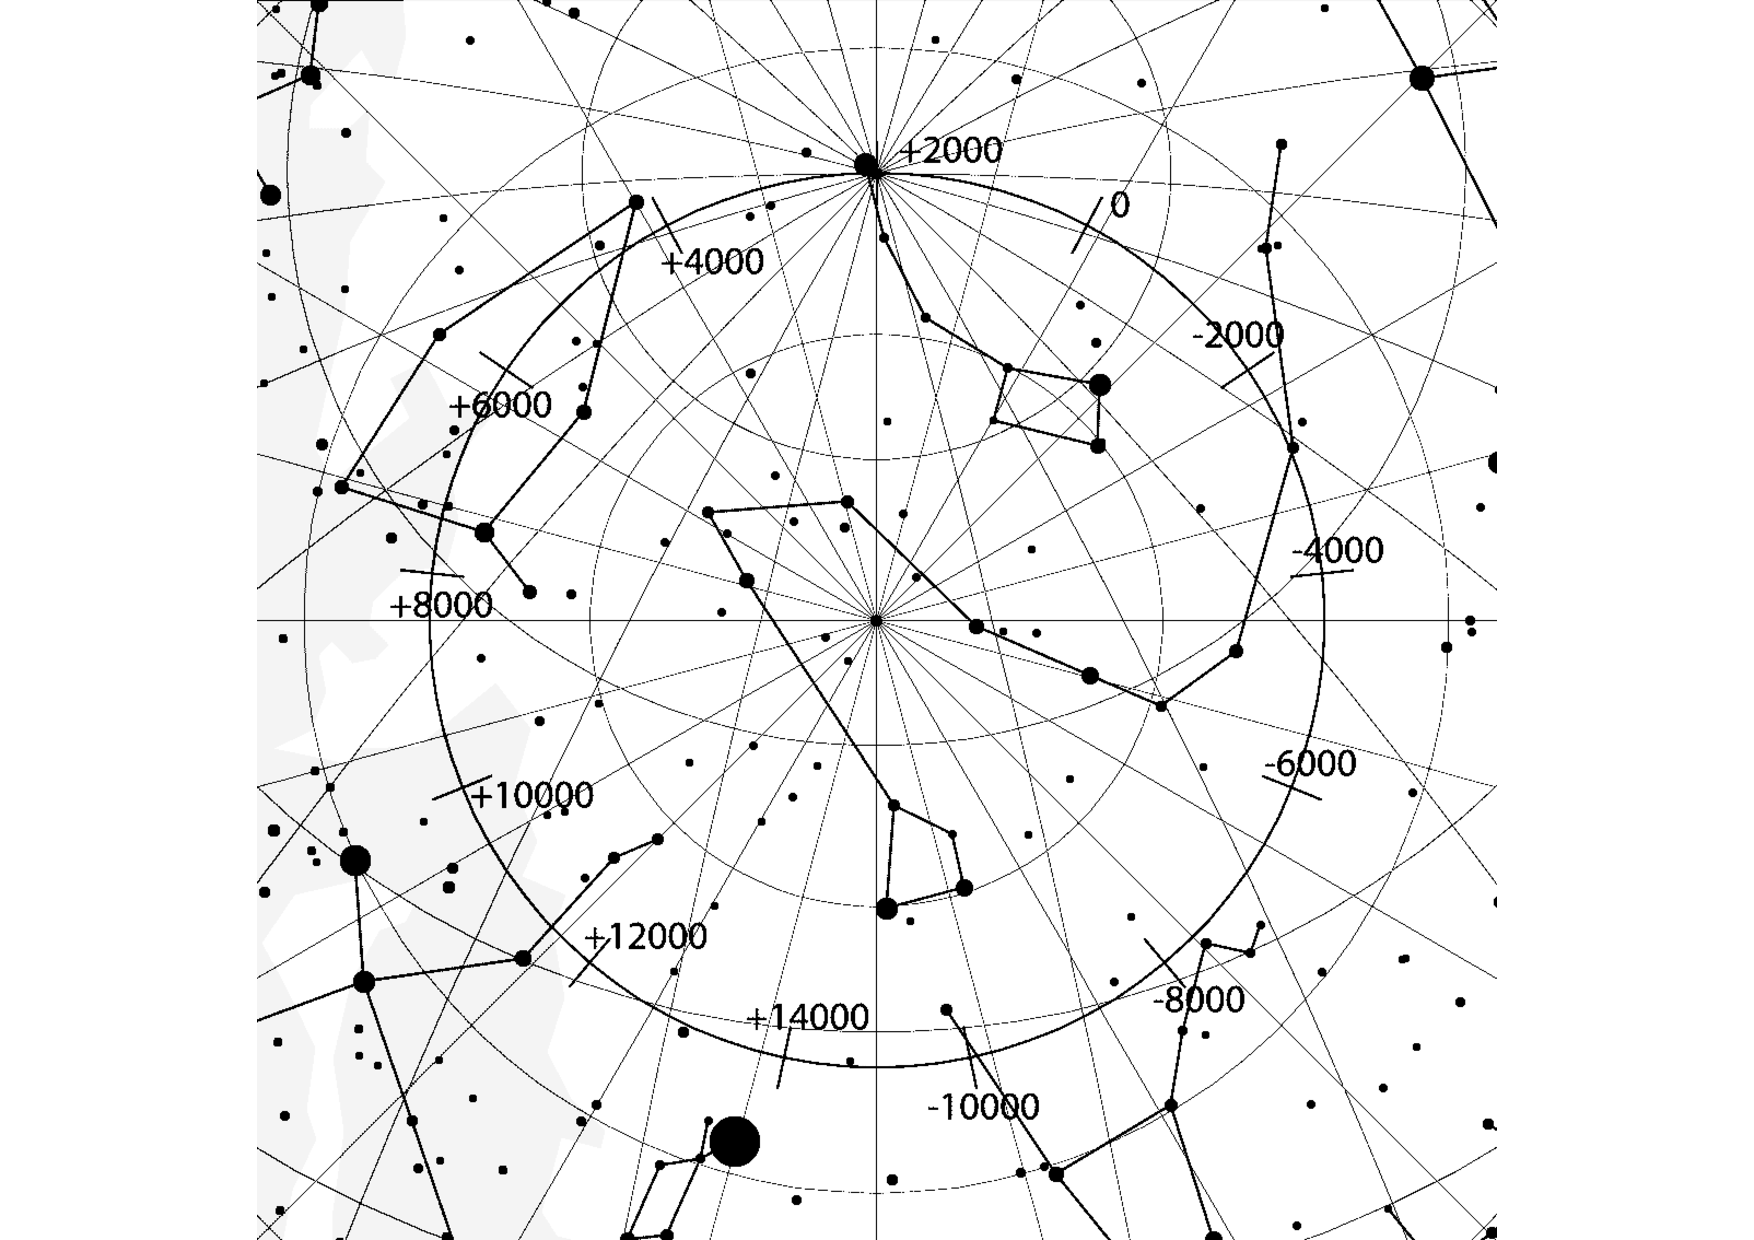
\includegraphics[width = .5\tw]{precession.pdf}
	\caption{Прецессионное движение северного полюса мира}
	\label{fig:precession-path}
\end{wrapfigure}
Поворот оси Земли имеет различные последствия. Во-первых, меняется продолжительность тропического года, он становится примерно на $20$~минут короче звёздного. Во-вторых, из-за прецессии меняется вид звёздного неба, хоть и происходит это очень медленно (см.~Рис.\,\ref{fig:precession-path}).